% --- Applications (from sections/diffusion/complete/applications.tex) ---
\section{Applications}
\begin{frame}{}
    \LARGE Diffusion Models: \textbf{Applications}
\end{frame}

% --- GLIDE (from sections/diffusion/complete/applications/glide.tex) ---
\begin{frame}{Application: GLIDE - OpenAI}
\begin{figure}
    \centering
    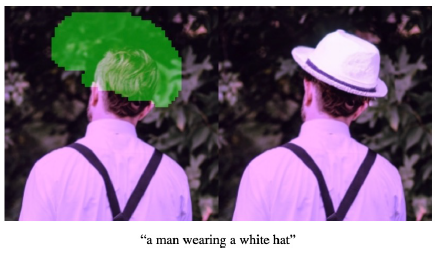
\includegraphics[height=0.8\textheight, width=\textwidth, keepaspectratio]{images/diffusion/diff_results_2.png}
    \caption*{Image Inpainting with GLIDE}
\end{figure}
\footnotetext{\href{https://arxiv.org/abs/2112.10741}{GLIDE: Towards Photorealistic Image Generation and Editing with Text-Guided Diffusion Models}}
\end{frame}

% --- DALL·E 2 (from sections/diffusion/complete/applications/dalle2.tex) ---
\begin{frame}{Application: DALL.E 2 - OpenAI}
\begin{figure}
    \centering
    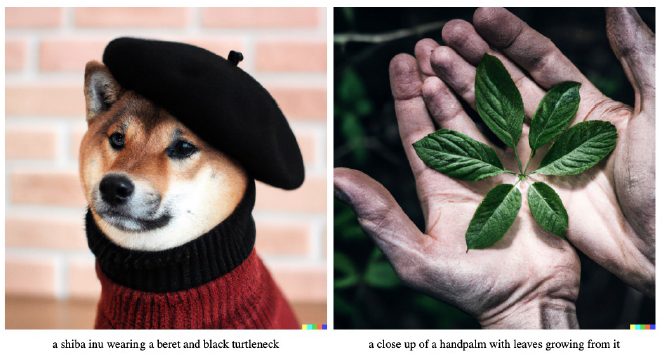
\includegraphics[height=0.8\textheight, width=\textwidth, keepaspectratio]{images/diffusion/diff_results_3.png}
    \caption*{Text to image generation eith DAll.E 2}
\end{figure}
\footnotetext{\href{https://arxiv.org/abs/2204.06125}{Hierarchical Text-Conditional Image Generation with CLIP Latents}}
\end{frame}

\begin{frame}{DALL.E 2 - OpenAI}
\begin{figure}
    \centering
    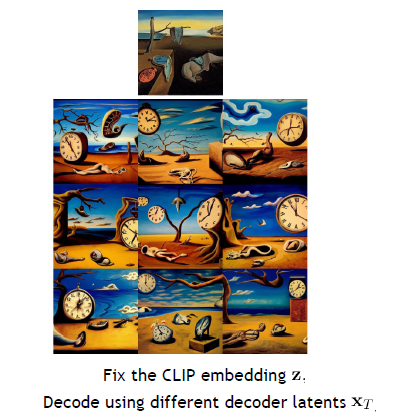
\includegraphics[height=0.8\textheight, width=\textwidth, keepaspectratio]{images/diffusion/diff_results_4.png}
    \caption*{Image Variations}
\end{figure}

\footnotetext{\href{https://arxiv.org/abs/2204.06125}{Hierarchical Text-Conditional Image Generation with CLIP Latents}}


\end{frame}

\begin{frame}{DALL.E 2 - OpenAI}
\begin{figure}
    \centering
    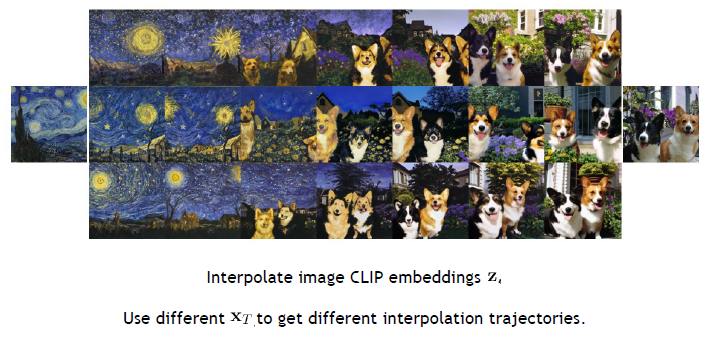
\includegraphics[height=0.8\textheight, width=\textwidth, keepaspectratio]{images/diffusion/diff_results_5.png}
    \caption*{Image interpolation}
\end{figure}

\footnotetext{\href{https://arxiv.org/abs/2204.06125}{Hierarchical Text-Conditional Image Generation with CLIP Latents}}

\end{frame}

\begin{frame}{DALL.E 2 - OpenAI}
\begin{figure}
    \centering
    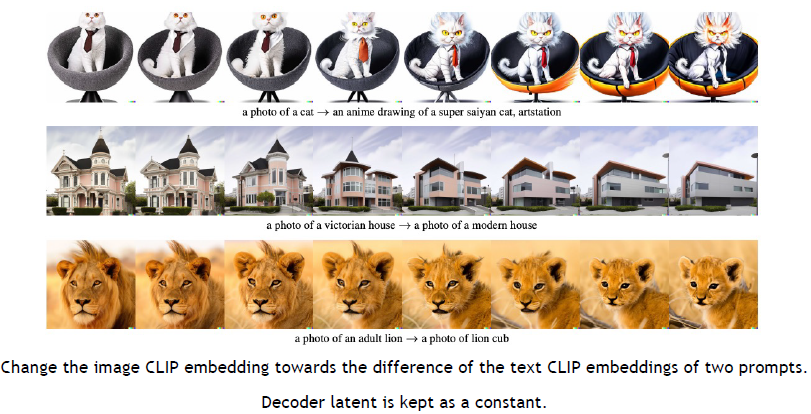
\includegraphics[height=0.8\textheight, width=\textwidth, keepaspectratio]{images/diffusion/diff_results_6.png}
    \caption*{Text Difference Image interpolation}
\end{figure}

\footnotetext{\href{https://arxiv.org/abs/2204.06125}{Hierarchical Text-Conditional Image Generation with CLIP Latents}}

\end{frame}

% --- Imagen (from sections/diffusion/complete/applications/imagen.tex) ---
\begin{frame}{Imagen - Google}

\begin{figure}
    \centering
    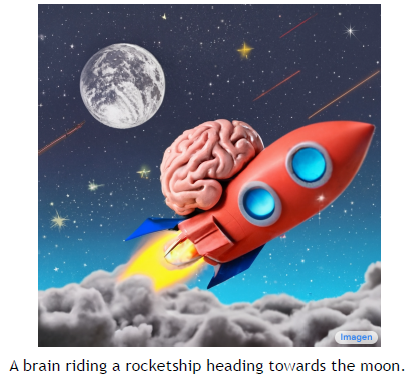
\includegraphics[height=0.8\textheight, width=\textwidth, keepaspectratio]{images/diffusion/diff_results_7.png}
\end{figure}

\footnotetext{\href{https://arxiv.org/abs/2205.11487}{Photorealistic Text-to-Image Diffusion Models with Deep Language Understanding}}
\end{frame}

\begin{frame}{Imagen - Google}

\begin{figure}
    \centering
    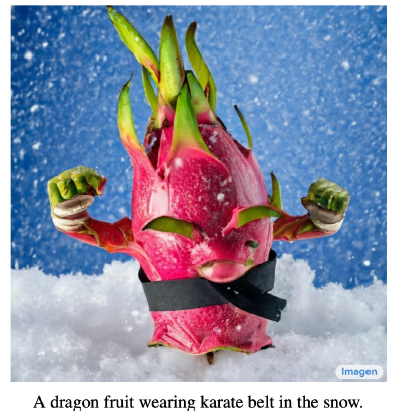
\includegraphics[height=0.8\textheight, width=\textwidth, keepaspectratio]{images/diffusion/diff_results_8.png}
\end{figure}

\footnotetext{\href{https://arxiv.org/abs/2205.11487}{Photorealistic Text-to-Image Diffusion Models with Deep Language Understanding}}
\end{frame}

\begin{frame}{Imagen - Google}

\begin{figure}
    \centering
    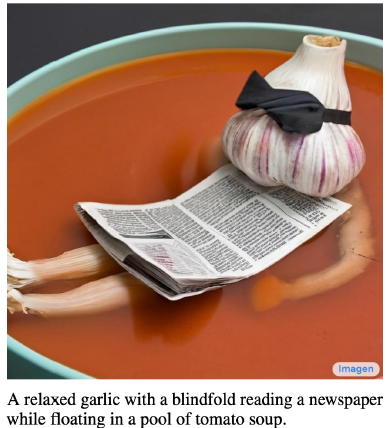
\includegraphics[height=0.8\textheight, width=\textwidth, keepaspectratio]{images/diffusion/diff_results_9.png}
\end{figure}

\footnotetext{\href{https://arxiv.org/abs/2205.11487}{Photorealistic Text-to-Image Diffusion Models with Deep Language Understanding}}
\end{frame}

% --- Nano Banana 2 (Google DeepMind blog, Feb 2026) ---
\begin{frame}[t]{Application: Nano Banana 2 -- Google DeepMind}
    \begin{figure}
        \centering
        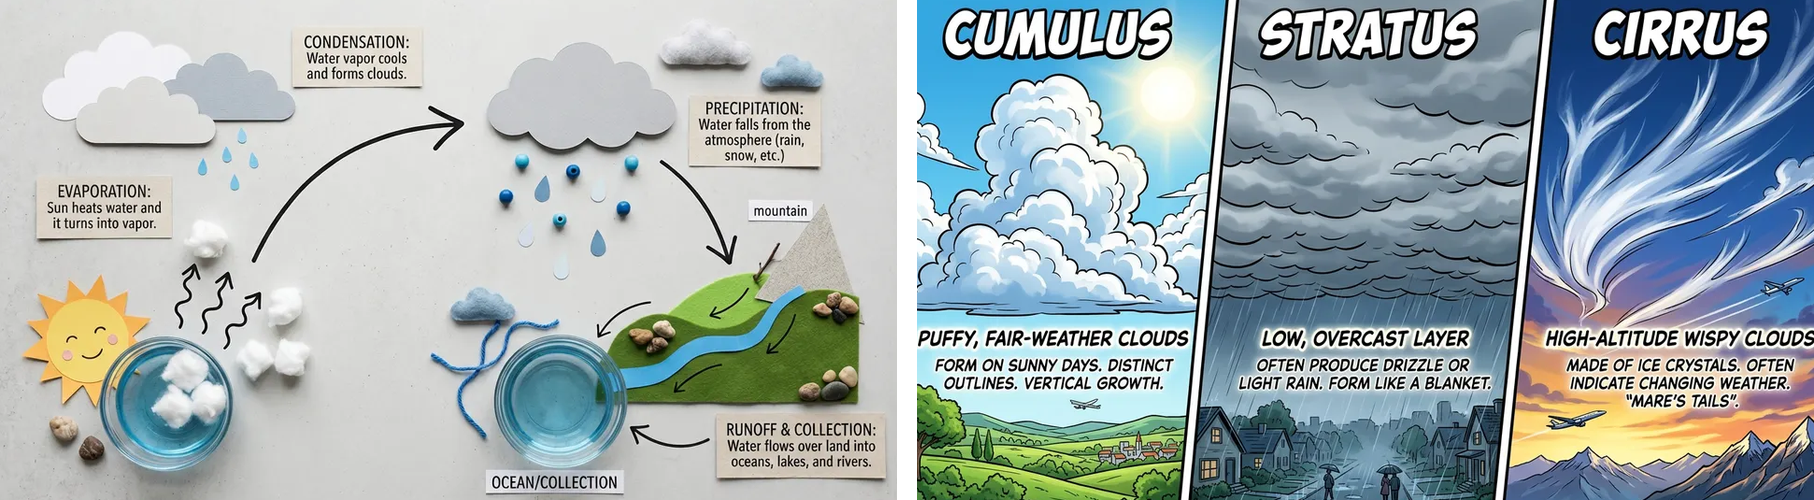
\includegraphics[width=\linewidth,keepaspectratio]{assets/New-Lecture-Stable_Diffusion/nano-banana-2/slide1_world_knowledge.png}
        \caption*{Examples: water-cycle infographic and cloud-type comparison.}
    \end{figure}
    \footnotetext{\href{https://blog.google/innovation-and-ai/technology/ai/nano-banana-2/}{Raisinghani, ``Nano Banana 2: Combining Pro capabilities with lightning-fast speed,'' Google DeepMind blog (Feb 2026).}}
    \begin{itemize}
        \item Builds on Google's Gemini Image line: Nano Banana (2025) $\rightarrow$ Nano Banana Pro $\rightarrow$ Nano Banana 2.
        \item Production-ready output: multiple aspect ratios and resolutions from 512px to 4K.
    \end{itemize}
\end{frame}

% --- Diffusion Autoencoders (from sections/diffusion/complete/applications/dae.tex) ---
\begin{frame}{Diffusion Autoencoders}

\begin{figure}
    \centering
    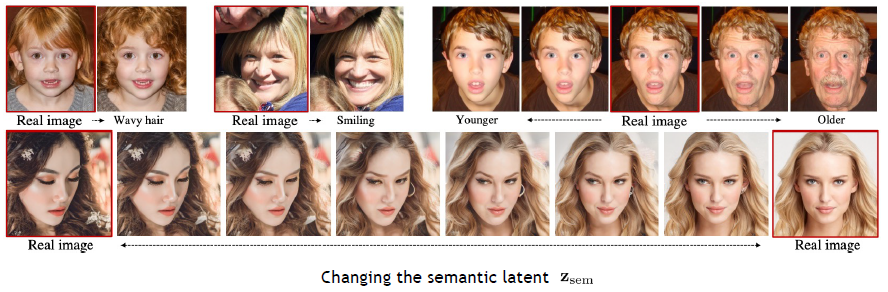
\includegraphics[height=0.8\textheight, width=\textwidth, keepaspectratio]{images/diffusion/diff_results_10.png}
    \caption*{Learning semantic meaningful latent representations in diffusion models}
\end{figure}

\footnotetext{\href{https://arxiv.org/abs/2111.15640}{Diffusion Autoencoders: Toward a Meaningful and Decodable Representation}}
\end{frame}

% --- Super Resolution (from sections/diffusion/complete/applications/super-resolution.tex) ---
\begin{frame}{Super Resolution}

\begin{figure}
    \centering
    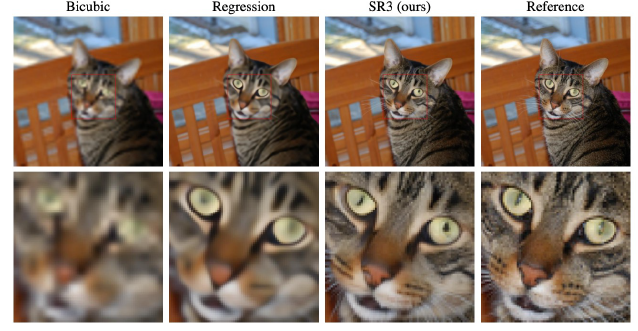
\includegraphics[height=0.8\textheight, width=\textwidth, keepaspectratio]{images/diffusion/diff_results_11.png}
    \caption*{Natural Image Super Resolution $64 \times 64 \longrightarrow 256 \times 256$}
\end{figure}

\footnotetext{\href{https://arxiv.org/abs/2104.07636}{Image Super-Resolution via Iterative Refinement}}
\end{frame}

% --- 3D Shape Generation (from sections/diffusion/complete/applications/3d-shape-generation.tex) ---
\begin{frame}{3D Shape Generation}

\begin{figure}
    \centering
    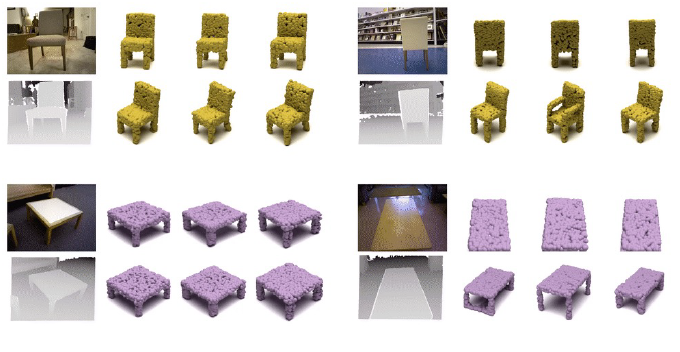
\includegraphics[height=0.8\textheight, width=\textwidth, keepaspectratio]{images/diffusion/diff_results_12.png}
\end{figure}

\footnotetext{\href{https://arxiv.org/abs/2104.03670}{3D Shape Generation and Completion through Point-Voxel Diffusion}}
\end{frame}

\begin{frame}{Try It Yourself!}
\centering
Text to Image generation with stable diffusion.
\centering
\href{https://huggingface.co/spaces/stabilityai/stable-diffusion}{https://huggingface.co/spaces/stabilityai/stable-diffusion}

\footnotetext{\href{https://arxiv.org/abs/2112.10752}{High-Resolution Image Synthesis with Latent Diffusion Models}}
\end{frame}
